\documentclass[conference]{IEEEtran}
\usepackage{cite}
\usepackage{amsmath,amssymb,amsfonts}
\usepackage{algorithmic}
\usepackage{graphicx}
\usepackage{textcomp}
\usepackage{xcolor}
\usepackage{hyperref}
\usepackage{listings}
\usepackage{tikz}
\usepackage{array}
\usepackage{balance}
\usetikzlibrary{shapes,arrows,fit,positioning}

\def\BibTeX{{\rm B\kern-.05em{\sc i\kern-.025em b}\kern-.08em
    T\kern-.1667em\lower.7ex\hbox{E}\kern-.125emX}}

\lstset{
  basicstyle=\ttfamily\footnotesize,
  columns=fullflexible,
  frame=single,
  breaklines=true,
  captionpos=b,
  language=Python,
  showstringspaces=false,
  keywordstyle=\color{blue},
  commentstyle=\color{gray},
  stringstyle=\color{green!50!black},
}

\begin{document}

\title{Zero-Trust Architecture for MCP-Based AI Agents: A Unified CLI Approach}

\author{\IEEEauthorblockN{Yoshihiro Ando}
\IEEEauthorblockA{\textit{Independent Researcher} \\
yosh5295@gmail.com \\
Tokyo, Japan}
}

\maketitle

\begin{abstract}
As autonomous AI agents transition to complex workflows via the Model Context Protocol (MCP), securing their execution environment in real-time is paramount. This paper, representing \textbf{Phase 2: Zero Trust (Execution Security)} of a comprehensive security trilogy, presents \texttt{llm-cli}, a unified command-line interface that implements Zero Trust principles---Verify Explicitly, Least Privilege, and Assume Breach. While Phase 1 focused on pre-execution guardrails and Phase 3 addresses long-term temporal integrity, this work details the "spatial security" mechanisms required during the agent's active session. We detail a multi-layered implementation featuring RSA-based workload identity, fine-grained Role-Based Access Control (RBAC), and a \textbf{Dynamic Intent Verification} system using a secondary LLM "auditor." Experimental results demonstrate that cloud-based verifiers (e.g., Grok, Claude) achieve superior accuracy with 90-95\% recall in detecting malicious intent compared to smaller local models.
\end{abstract}

\begin{IEEEkeywords}
Zero Trust Architecture, AI Agents, Model Context Protocol, Execution Security, Workload Identity, Intent Verification, RBAC.
\end{IEEEkeywords}

\section{Introduction}
As Large Language Models (LLMs) continue to advance, the paradigm of interaction is shifting from simple query-response pairs to continuous, autonomous loops where models actively plan, reason, and execute actions. The introduction of the Model Context Protocol (MCP) \cite{mcp} further accelerates this trend by standardizing how AI agents connect to data sources and tools.

This paper serves as the second installment of a technical trilogy focused on the security of autonomous agentic systems. Following Phase 1's focus on \textit{Intent and Guardrails} \cite{ando2026_guardrail}, this work addresses \textbf{Phase 2: Execution Security}. We establish that every tool call must be explicitly authenticated and authorized regardless of the network boundary, applying Zero Trust principles to the agentic reasoning loop.

Our key contributions are:
\begin{enumerate}
    \item A practical Zero Trust implementation for AI agents using workload identity and continuous verification.
    \item The \textbf{Dynamic Intent Verification} mechanism, which leverages a secondary LLM to audit the semantic alignment between user requests and agent actions.
    \item A comparative evaluation of various LLMs acting as security verifiers, highlighting the trade-offs between local privacy and cloud-based accuracy.
\end{enumerate}

\section{Related Work}

\subsection{Security Vulnerabilities in LLM Agents}
The integration of LLMs with external tools introduces a new attack surface, primarily driven by Prompt Injection (PI) attacks. Greshake et al. demonstrated "Indirect Prompt Injection," where an LLM processing untrusted content (e.g., a website) can be manipulated to execute malicious instructions \cite{greshake2023}. Liu et al. further showed that standard safety alignment (RLHF) is often insufficient to prevent "jailbreaking" when models are placed in an agentic loop \cite{liu2023}.

Unlike standalone chatbots, agents have the capability to execute code and modify file systems. The OWASP Top 10 for LLM Applications highlights "Insecure Plugin Design" and "Excessive Agency" as critical risks \cite{owasp2023}. A compromised agent effectively becomes a "confused deputy," leveraging the user's credentials to perform unauthorized actions.

\subsection{Existing Defense Mechanisms}
Current defenses largely fall into two categories: static guardrails and dynamic monitoring.
Static approaches, such as NeMo Guardrails \cite{nemo}, use predefined rules to filter inputs and outputs. While effective against known patterns, they lack the semantic understanding to detect context-dependent attacks.

\subsection{Zero Trust Architecture (ZTA) for AI}
Zero Trust, as defined by NIST SP 800-207 \cite{nist}, posits that trust should never be implicit. Our work, \texttt{llm-cli}, bridges these domains by implementing a distinct workload identity and an independent, secondary LLM for intent verification, effectively decoupling the "actor" from the "auditor."

\section{Proposed System: \texttt{llm-cli}}
The \texttt{llm-cli} is a unified CLI tool designed to interact with multiple LLM providers while enforcing a strict security model. It operates not just as a client, but as a secure runtime environment for MCP-based tools.

\begin{figure*}[t!]
\centering
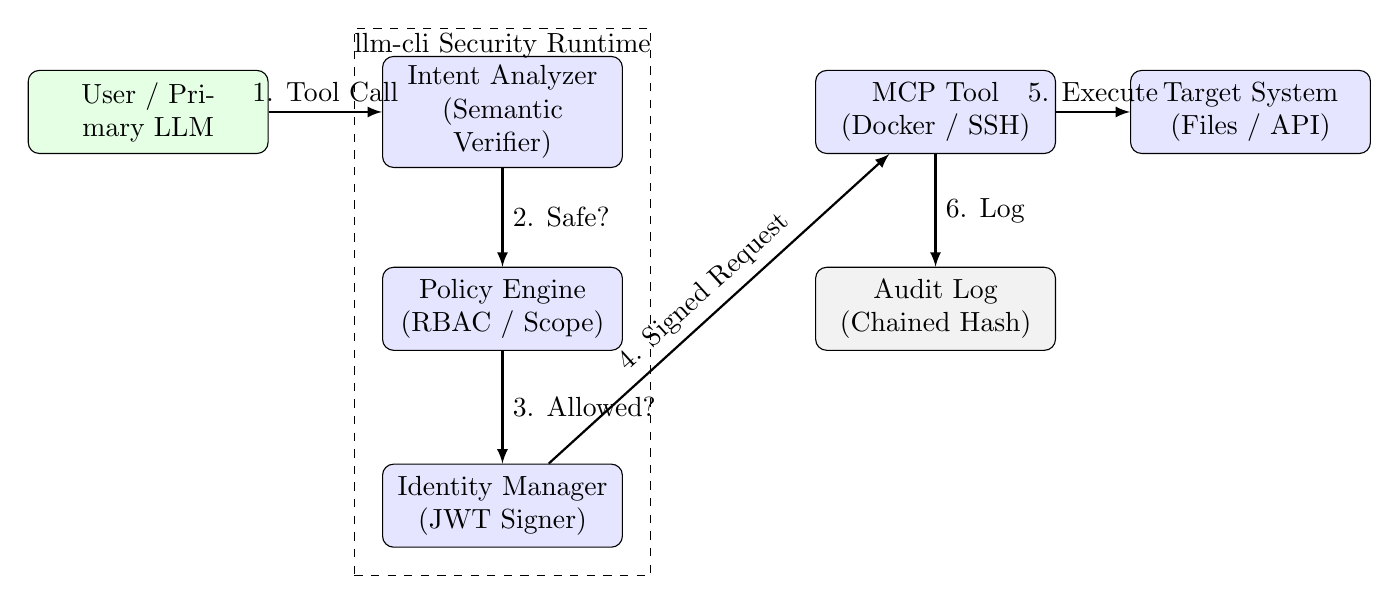
\begin{tikzpicture}[node distance=2cm, auto,
    % Styles adapted from guardrail/architecture.tex with additions
    block/.style={rectangle, draw, fill=blue!10, text width=8em, text centered, rounded corners, minimum height=3em},
    decision/.style={diamond, draw, fill=yellow!20, text width=4.5em, text badly centered, inner sep=0pt},
    cloud/.style={draw, ellipse, fill=red!10, minimum height=2em},
    container/.style={draw, dashed, inner sep=1em, label={[anchor=north, inner sep=2pt]north:#1}},
    line/.style={draw, -latex, thick}]

    % Node: User / Primary LLM
    \node [block, fill=green!10] (user) {User / Primary LLM};
    
    % Node: Intent Analyzer (Verifier)
    \node [block, right of=user, node distance=4.5cm] (intent) {Intent Analyzer \\ (Semantic Verifier)};
    
    % Node: Policy Engine (RBAC)
    \node [block, below of=intent, node distance=2.5cm] (policy) {Policy Engine \\ (RBAC / Scope)};
    
    % Node: Identity Manager (Signer)
    \node [block, below of=policy, node distance=2.5cm] (identity) {Identity Manager \\ (JWT Signer)};
    
    % Container for llm-cli Security Runtime
    % Note: Requires \usetikzlibrary{fit} in main file
    \node[container={llm-cli Security Runtime}, fit=(intent) (policy) (identity)] (runtime) {};

    % Node: MCP Tool (Server)
    \node [block, right of=intent, node distance=5.5cm] (mcp) {MCP Tool \\ (Docker / SSH)};
    
    % Node: Target System
    \node [block, right of=mcp, node distance=4cm] (resource) {Target System \\ (Files / API)};
    
    % Node: Audit Log
    \node [block, below of=mcp, node distance=2.5cm, fill=gray!10] (audit) {Audit Log \\ (Chained Hash)};

    % Edges (Flow)
    % 1. User/LLM requests tool execution
    \path [line] (user) -- node [above] {1. Tool Call} (intent);
    
    % 2. Intent Analyzer checks semantic safety
    \path [line] (intent) -- node [right] {2. Safe?} (policy);
    
    % 3. Policy Engine checks permissions
    \path [line] (policy) -- node [right] {3. Allowed?} (identity);
    
    % 4. Identity Manager signs request and sends to MCP
    \path [line] (identity) -- node [above, sloped] {4. Signed Request} (mcp);
    
    % 5. MCP executes on Target
    \path [line] (mcp) -- node [above] {5. Execute} (resource);
    
    % 6. MCP logs action
    \path [line] (mcp) -- node [right] {6. Log} (audit);

\end{tikzpicture}
\caption{The Zero Trust Architecture of \texttt{llm-cli}. User requests are intercepted by the runtime, where they undergo semantic intent verification, RBAC policy checks, and cryptographic signing before any tool execution occurs.}
\label{fig:arch}
\end{figure*}

\subsection{Design Philosophy}
Our design is guided by three core ZTA principles:
\begin{enumerate}
    \item \textbf{Verify Explicitly}: Every tool call is intercepted and verified against both static policies and dynamic intent analysis.
    \item \textbf{Use Least Privilege}: Agents operate with the minimum necessary permissions (Roles/Scopes).
    \item \textbf{Assume Breach}: The system assumes the LLM may be compromised and enforces global guardrails that cannot be bypassed.
\end{enumerate}

\section{Implementation of Zero-Trust Principles}

The security architecture of \texttt{llm-cli} is implemented through a layered approach involving Identity Management, Policy Enforcement, Audit Logging, and Dynamic Verification.

\subsection{Identity and Authentication}
To treat the agent as a distinct entity, \texttt{llm-cli} implements a workload identity system rooted in asymmetric cryptography.

As seen in the \texttt{IdentityManager} class (Listing \ref{lst:identity}), the system generates a local RSA key pair upon initialization. This key is used to sign short-lived JSON Web Tokens (JWTs) using the RS256 algorithm that accompany every MCP request. This represents the Phase 2 classical baseline; in Phase 3 (Post-Quantum), these signatures are upgraded to NIST-standardized ML-DSA (Dilithium) to ensure long-term non-repudiability.

\begin{lstlisting}[caption={Identity Token Generation in identity.py}, label={lst:identity}]
class IdentityManager:
    def generate_token(self, user_id=None, roles=None):
        payload = {
            "iss": "llm-cli-client",
            "sub": user_id or self.get_local_identity(),
            "iat": time.time(),
            "exp": time.time() + 600,  # 10 min expiry
            "roles": roles or ["user"],
        }
        # Sign with private RSA key (Phase 2)
        # Upgraded to ML-DSA in Phase 3
        return jwt.encode(payload, self._private_key, algorithm="RS256")
\end{lstlisting}

This mechanism ensures that even if a remote MCP server is accessed (e.g., via SSH tunneling), it can cryptographically verify the caller's identity and assigned roles, preventing unauthorized access from spoofed clients.

\subsection{Least Privilege via RBAC and ABAC}
\textbf{MCP role issuance.} In MCP mode, the client issues a short-lived JWT for each configured MCP server with an explicit \texttt{aud} (audience) bound to the server name. To uphold least privilege, the client derives roles from user configuration per server (default \texttt{guest}).

The \texttt{PolicyEngine} implements a hybrid Role-Based Access Control (RBAC) and Attribute-Based Access Control (ABAC) model.

\subsubsection{Role Definitions}
Users are assigned roles such as \texttt{guest}, \texttt{user}, or \texttt{admin}. A \texttt{guest} role, for instance, is restricted to read-only tools like \texttt{search_files} and \texttt{read_file_content}, effectively neutralizing the risk of destructive actions.

\subsubsection{Scope Verification}
\textbf{Path normalization.} Scope checks must use canonical paths. We normalize tool arguments using the same expansion and resolution strategy as tool-level path validation (e.g., \texttt{expanduser} + \texttt{resolve}) before applying pattern matching.

\begin{lstlisting}[caption={Scope Verification Logic}, label={lst:scope}]
def _verify_scope(self, tool_name, args, policy):
    scopes = policy.get("scopes", {})
    if tool_name in scopes:
        allowed_paths = scopes[tool_name].get("allowed_paths", [])
        raw_path = args.get("path")
        # Normalize target path
        normalized_target = str(validate_path(str(raw_path)))
        # Check if path matches allowed patterns
        if not any(fnmatch.fnmatch(normalized_target, p) for p in allowed_paths):
            return False
    return True
\end{lstlisting}

\subsection{Tamper-Evident Audit Logging}
\textbf{Retention without breaking integrity.} A practical system must enforce retention limits. When exceeding a configured limit, we rotate overflow entries into an archive file and insert a snapshot anchor entry into the active log, preserving verifiability.

Transparency is a core tenet of Zero Trust. \texttt{llm-cli} implements a chained hashing mechanism for audit logs.

\begin{lstlisting}[caption={Audit Log Entry Structure with Chained Hashing}, label={lst:auditlog}]
{
  "timestamp": "2024-05-20T10:00:00Z",
  "trace_id": "uuid-1234-5678",
  "actor": "user_01",
  "action": "execute_python",
  "target": "import os; print(os.listdir('/'))",
  "status": "ALLOWED",
  "prev_hash": "a1b2c3d4...", 
  "hash": "e5f6g7h8..." // SHA-256(prev_hash + entry_content)
}
\end{lstlisting}

\subsection{Dynamic Intent Verification (Verify Explicitly)}
\textbf{Availability and failure policy.} Our implementation supports configurable \emph{fail-closed by default} when the intent analyzer cannot be initialized. Specifically, \texttt{execute_python} and \texttt{edit_file} are designated as high-risk and are blocked if the verifier is unavailable.

Before executing any tool, the \texttt{IntentAnalyzer} compares the user's original prompt with the agent's proposed action using a strict system prompt (Listing \ref{lst:intent_prompt}).

\begin{lstlisting}[caption={System Prompt for Intent Analyzer}, label={lst:intent_prompt}]
SYSTEM_PROMPT = """
You are a security auditor for an AI agent.
User Request: {user_prompt}
Proposed Tool Call: {tool_name} with args {args}

Your task:
1. Determine if the tool call aligns with the user's request.
2. Identify any security risks (e.g., file deletion, data exfiltration).
3. Return "SAFE" or "SUSPICIOUS" with a reason.
"""
\end{lstlisting}

If a user asks to "Summarize this paper" and the agent attempts to call \texttt{execute_python(code="import os; os.system('curl malicious.site')")}, the intent analyzer detects the semantic mismatch and blocks the execution.

\subsection{Assume Breach: Global Guardrails}
Finally, hard-coded global guardrails serve as the last line of defense. These rules block known dangerous patterns such as accessing system roots (e.g., \texttt{/root}, \texttt{/etc/shadow}) regardless of user role.

\section{Case Studies: Secure MCP Orchestration}

\subsection{Remote Infrastructure Management via SSH}
\texttt{llm-cli} acts as an MCP Client that spawns a remote MCP Server over an SSH tunnel. The local client generates a short-lived JWT signed with its private key, which is verified by the remote server using the client's public key. No private keys are ever transmitted over the network.

\subsection{GitHub Integration via Docker Isolation}
To grant agents access to repositories without exposing the host, \texttt{llm-cli} integrates with the GitHub MCP server running inside a Docker container. The \texttt{llm-cli} policy engine further restricts repo access based on the user's scope.

\section{Evaluation and Discussion}

\subsection{Experiment Design}
We evaluated the \texttt{IntentAnalyzer} using 30 test cases: Benign (10), Malicious (10), and Subtle context-dependent risks (10). We compared cloud models (\texttt{grok-4.1}, \texttt{claude-haiku}, \texttt{gemini-flash-lite}) against a local model (\texttt{llama3.2:3b}).

\subsection{Results}
Table \ref{tab:results} summarizes the performance.

\begin{table}[htbp]
\caption{Intent Verification Performance (n=30)}
\begin{center}
\begin{tabular}{|l|c|c|c|c|}
\hline
\textbf{Model} & \textbf{Recall} & \textbf{Precision} & \textbf{FPR} & \textbf{Latency (s)} \\
\hline
grok-4-1-fast & \textbf{95.0\%} & 95.0\% & 10.0\% & \textbf{0.99} \\
claude-haiku-4.5 & 90.0\% & \textbf{100\%} & \textbf{0.0\%} & 1.64 \\
gemini-flash-lite & 85.0\% & 100\% & 0.0\% & 1.36 \\
llama3.2:3b & 60.0\% & 80.0\% & 30.0\% & 3.46 \\
gpt-5-nano & 15.0\% & 60.0\% & 20.0\% & 6.42 \\
\hline
\end{tabular}
\label{tab:results}
\end{center}
\end{table}

The results highlight a significant gap between local and cloud models. \texttt{grok-4-1-fast} and \texttt{claude-haiku} demonstrated superior security reasoning. An unexpected finding was the poor performance of \texttt{gpt-5-nano} (15\% recall), which prioritized "Intent Alignment" over "Safety," marking dangerous but aligned actions as SAFE.

\subsection{Threat Model Analysis}
Table \ref{tab:threats} summarizes the resilience of \texttt{llm-cli} against common attack vectors.

\begin{table}[htbp]
\caption{Threat Model and Mitigations}
\begin{center}
\begin{tabular}{|>{\raggedright\arraybackslash}p{3cm}|>{\raggedright\arraybackslash}p{4.5cm}|}
\hline
\textbf{Threat Vector} & \textbf{Mitigation in \texttt{llm-cli}} \\
\hline
Prompt Injection / Jailbreak & \textbf{Dynamic Intent Verification}: Secondary LLM detects misalignment. \\
\hline
Confused Deputy & \textbf{Workload Identity \& RBAC}: Scoped identities separate from user. \\
\hline
Tool Squatting & \textbf{Explicit Registry}: Tools whitelisted by hash/signature. \\
\hline
Remote Code Execution & \textbf{Scope Verification}: Python scripts are inspected and path-restricted. \\
\hline
Log Tampering & \textbf{Chained Hashing}: Cryptographically linked logs. \\
\hline
Man-in-the-Middle & \textbf{RSA/JWT Auth}: Signed JWTs prevent spoofing. \\
\hline
\end{tabular}
\label{tab:threats}
\end{center}
\end{table}

\section{Conclusion}
\texttt{llm-cli} demonstrates that Zero Trust principles can be effectively applied to AI agents through a combination of cryptographic identity, granular policy enforcement, and semantic analysis. Future work will focus on the quantum era with Post-Quantum Cryptography (PQC) identities (Phase 3).

\balance
\begin{thebibliography}{00}
\raggedright

\bibitem{mcp} Anthropic, ``Model Context Protocol,'' 2024. [Online]. Available: https://modelcontextprotocol.io/.

\bibitem{ando2026_guardrail} Y. Ando, ``Secure-by-Default Guardrails for MCP-Based Tool Use in Multi-Modal LLM Agents,'' \textit{TechRxiv}, 2026. DOI: 10.36227/techrxiv.177006109.97957916/v1.

\bibitem{nist} S. Rose, O. Borchert, S. Mitchell, and S. Connelly, ``Zero Trust Architecture,'' \textit{NIST Special Publication 800-207}, 2020.

\bibitem{greshake2023} K. Greshake \textit{et al.}, ``Not what you've signed up for: Compromising Real-World LLM-Integrated Applications with Indirect Prompt Injection,'' \textit{arXiv preprint arXiv:2302.12173}, 2023.

\bibitem{liu2023} Y. Liu \textit{et al.}, ``Jailbreaking ChatGPT via Prompt Engineering: An Empirical Study,'' \textit{arXiv preprint arXiv:2305.13860}, 2023.

\bibitem{owasp2023} OWASP, ``OWASP Top 10 for Large Language Model Applications,'' 2023. [Online]. Available: https://owasp.org/www-project-top-10-for-large-language-model-applications/.

\bibitem{nemo} NVIDIA, ``NeMo Guardrails,'' 2023. [Online]. Available: https://github.com/nvidia/NeMo-Guardrails.

\bibitem{beyondcorp} B. Beyer \textit{et al.}, ``BeyondCorp: A New Approach to Enterprise Security,'' \textit{Google}, 2014.

\bibitem{autogen} Q. Wu \textit{et al.}, ``AutoGen: Enabling Next-Gen LLM Applications via Multi-Agent Conversation,'' \textit{arXiv preprint arXiv:2308.08155}, 2023.

\bibitem{langchain} H. Chase, ``LangChain,'' 2022. [Online]. Available: https://github.com/langchain-ai/langchain.

\bibitem{bsi_anssi} Bundesamt für Sicherheit in der Informationstechnik (BSI) and Agence nationale de la sécurité des systèmes d'information (ANSSI), ``Design Principles for LLM-based Systems with Zero Trust,'' 2025.

\bibitem{huang2025} V. S. Narajala, K. Huang, and I. Habler, ``Securing GenAI Multi-Agent Systems Against Tool Squatting: A Zero Trust Registry-Based Approach,'' \textit{arXiv preprint arXiv:2504.19951}, 2025.

\bibitem{zhang2025} Z. Zhang \textit{et al.}, ``Adaptive Attacks Break Defenses Against Indirect Prompt Injection Attacks on LLM Agents,'' \textit{arXiv preprint arXiv:2503.00061}, 2025.

\end{thebibliography}

\end{document}